\documentclass{article}

\usepackage[brazil]{babel}
\usepackage[utf8]{inputenc}
\usepackage[T1]{fontenc}% optional T1 font encoding
\usepackage[%
    colorlinks=true,
    pdfborder={0 0 0},
    linkcolor=red
]{hyperref}
\usepackage[all]{hypcap}
\usepackage{amsmath}
\interdisplaylinepenalty=2500
\usepackage{graphicx}
\usepackage[cmintegrals]{newtxmath}
\usepackage{cite}
\usepackage{listings}
\usepackage{hyperref}
\usepackage{indentfirst}
\usepackage{siunitx}
\usepackage{textgreek}
\usepackage[portuguese,linesnumbered,ruled]{algorithm2e}
\usepackage{multirow}
\usepackage{anysize}

\begin{document}

\title{Diodos e Fontes de Tensão Contínua}
\author{Bianca Yoshie Itiroko - 164923 \\ Luiz Eduardo Cartolano - 183012 \\ Seong Eun Kim - 177143 \\ EE534 - Turma Y - Grupo 2}
\date{Setembro de 2018}

\maketitle

\begin{abstract}
Esse experimento tem como objetivo estudar as características do diodo em circuitos que culminam em uma fonte de tensão contínua. Através deles, pode-se observar o comportamento do diodo que não conduz abaixo de uma tensão limiar. Essa tensão é a tensão direta, no caso diodo comum, ou a tensão de Zener, no diodo Zener, para os quais obteve-se os valores de 0,7V e 0,6V, respectivamente. Além disso, pode-se observar uma aplicação do transistor para manter o diodo conduzindo independentemente da carga. 

\end{abstract}

\section{Introdução}
O diodo é um componente eletrônico composto de um cristal semicondutor de silício ou germânio cujas faces opostas são dopadas por diferentes materiais, o que gera uma polarização em cada uma das extremidades. Essa polarização faz com que seja permitido um sentido para passagem da corrente com muito mais facilidade do que pelo outro.

Das várias aplicações desse componente, pode-se destacar como a mais comum o projeto de circuitos retificadores. Estes são voltados para a conversão de corrente alternada em contínua e portanto de extrema importância para um desempenho mais eficaz de sistemas e aparelhos eletrônicos. Como a corrente distribuída pela rede elétrica é alternada, a conversão torna-se necessária pois aparelhos eletrônicos usuais exigem o uso de corrente contínua.

Nesse experimento, será estudada a aplicação do diodo voltado para a construção de uma fonte regulada de tensão contínua. Busca-se manusear e caracterizar esses componentes extraindo seus principais parâmetros. Para aproximar o experimento do que acontece em casos reais, utilizou-se um transformador como fornecedor da corrente alternada.

\section{Procedimentos}
Para a realização dos experimentos, utilizou-se de um transformador de $100V_{rms}$ para $9V_{rms}$ com tap central, dois diodos, um diodo Zener, um transistor, resistores de $220\Omega$, $910\Omega$ e $1,3K\Omega$ e capacitores eletrolíticos de $1000\mu$F e $2200\mu$F.

Primeiramente, usando um multímetro, verificou-se o funcionamento do transformador. Então, projetou-se um circuito de um diodo em série com um resistor de $1,3k\Omega$ e usou-se o transformador, com o terra no tap central, para alimentá-lo. Com a ajuda de um osciloscópio no modo XY, obteve-se a curva característica dos diodos (comum e Zener).

Na segunda parte do experimento, trocou-se a fonte de tensão alternada, provida pelo transformador, por uma fonte de tensão contínua. Inicialmente, colocou-se uma tensão de 9V e baixou-se alguns volts. Para cada valor de tensão, obteve-se as tensões no diodo e no resistor. Esse procedimento foi feito tanto para o diodo comum, como para o diodo Zener.

Na terceira parte do experimento, montou-se o circuito mostrado na Figura \ref{fig:circ1}. Para tal, os valores dos elementos foram previamente calculados no projeto do circuito: para a resistência, calculou-se que seria necessário $1202,7\Omega$ e para o capacitor, calculou-se que seria necessário $833\mu$F. Na construção do circuito usou-se um capacitor de $1000\mu$F e um resistor de $1,3K\Omega$. Com o circuito já montado, mediu-se a tensão de ripple, a tensão no capacitor e $v_{out}$. Depois, substituiu-se o capacitor de $1000\mu$F pelo de $2200\mu$F e fez-se as mesmas medições.

Para a quarta parte, projetou-se o circuito da Figura \ref{fig:circ2}. Para que a corrente sobre a carga fosse de 10mA, usou-se em R1 uma resistência de $220\Omega$ e em R2 uma resistência de $910\Omega$. Então, avaliou-se as formas de onda sobre o diodo e sobre a carga através do osciloscópio. Depois, trocou-se R2 por uma resistência de $220\Omega$ e fez-se as mesmas avaliações.

Para a quinta parte, retornou-se R2 para a carga original e, por fim, projetou-se o circuito da Figura \ref{fig:circ3}. Para definir as resistências, calculou-se os valores no projeto do circuito. Mediu-se as tensões no capacitor, no diodo Zener e na carga. Então, trocou-se o resistor de carga por um de menor resistência ($220\Omega$) e fez-se as mesmas medições.

\section{Discussão}
Na primeira parte do experimento, projetou-se um circuito de um diodo em série com um resistor e com um transformador para alimentá-lo. Ao ligar a saída do mesmo ao osciloscópio obteve-se o gráfico de tensão por corrente (usando-o no modo XY) no resistor da Figura \ref{fig:tensaoxcorrente}, de forma que pode-se ver que a corrente começa a passar apenas depois de aproximadamente 0,6V, o que é condizente com o valor teórico de 0,7V (no caso do diodo de silício).

Assim, pode-se chegar à tensão de Zener, isto é, a tensão no qual o diodo Zener entra em condução, que é justamente esse valor de aproximadamente de 0,6V. Para determinar a tensão de modo direto utilizou-se do mesmo método: também a partir do gráfico de tensão por corrente, encontrou-se o valor de aproximadamente 0,7V.

A principal motivação para realizar o experimento tanto com fontes de corrente contínua quanto alternada é poder estudar de maneira mais profunda o comportamento do diodo no circuito. Uma vez que se tem controle da tensão a ser aplicada no circuito pode-se fazer alguns testes com o mesmo. Primeiro, seria possível observar o comportamento do diodo para baixas tensões, isto é, próximo ao limiar. Além disso, é possível calcular o efeito resistivo do diodo no circuito, para isso, primeiro calcula-se os valores de tensão sobre o resistor e o diodo e, sabendo o valor da resistência, calcula-se a corrente do circuito. A partir da corrente, podemos achar o R{d} para cada uma das tensões escolhidas. Como podemos ver nas Tabelas \ref{tab: tensao-diodo} e \ref{tab: tensao-zener}. A partir dos dados de R{d}, foi possível plotar um gráfico, e usando a técnica dos mínimos quadrados encontrar a resistência média que o diodo exerce no circuito. Para o diodo comum encontrou-se o valor de $19,49\Omega$ e para o diodo de zener de $06,99\Omega$

Na segunda parte do experimento, montou-se o experimento da Figura \ref{fig:circ3}, que tem característica de retificador, isto é, transforma uma entrada de corrente alternada em uma saída de corrente contínua.

Com o auxílio do osciloscópio, mediu-se a tensão de ripple (tensão entre a carga e descarga do capacitor) e teve-se como valor encontrado 96mV, condizente com o esperado, uma vez que usou-se o valor de 100mV para tensão de ripple no projeto do circuito, podemos atribuir essa diferença de 4mV a mau contato dos cabos e o fato de que não trabalhou-se com componentes ideais.

Mediu-se também a tensão de saída e verificou-se que a mesma vale 10,6V e sua forma de onda é constante, assim como o esperado de um circuito retificador: o transformador fornece uma entrada alternada e tem-se por saída uma constante.

Em seguida substituiu-se o capacitor de $1000\mu$F pelo de $2200\mu$F e fez-se as mesmas medições. Dos dados coletados, houve alteração na tensão de ripple, cuja nova medida resultou em 60mV (cerca de 62,5 por cento do valor anterior), e nenhuma alteração tensão de saída, o que leva à conclusão que alterar o capacitor utilizado apenas altera o tempo com que o mesmo é carregado, mas não na saída do circuito no geral.

Para a quarta parte do experimento, montou-se o circuito da Figura \ref{fig:circ2}. Com o auxílio do osciloscópio, plotou-se a forma de onda sobre o capacitor e sobre a carga, obtendo ambas constantes de valor 12,4V e 11V, respectivamente (vide Figura \ref{fig:zenerNoRipple}). Diferentemente do circuito anterior, esse usa um diodo zener. Com valores suficientes de carga para que a tensão no diodo seja positiva, isto é, que ultrapasse o limiar do mesmo, ele faz com que não exista ripple na carga.

Ao trocar a carga por um resistor de impedância menor, pode-se notar que nessa nova configuração existe ripple na carga, cujo valor medido foi de 136mV (vide Figura \ref{fig:zenerRipple}). Isso pode ser explicado pois a soma de R1 com a tensão de zener deve ser igual a tensão no capacitor, então a tensão no diodo é diminuida e o limiar do diodo não é mais ultrapassado, assim ele fica desativado.

Para a quinta parte do experimento, inicialmente obteve-se as tensões de $13,1V$ no capacitor, $9,04V$ no Zener, $8,51V$ na carga. Depois trocou-se R2 para um valor menor e obteve-se as tensões de $13,1V$ no capacitor, $6,47V$ no Zener, $5,6V$ na carga. Se R2 tiver um valor muito pequeno, ele age como \textit{bypass} de D3 e a corrente passa por ele. A ddp em R2 e em D3 torna-se nula (diodo não conduz) e a ddp em R1 passa a ser a mesma de C1. Por isso colocou-se o transistor: para isolar a corrente que passa em R2. Assim, o diodo funciona independentemente da carga em R2.

\section{Conclusão}

Neste experimento, pode-se estudar as características e comportamento do diodo comum e de Zener através de circuitos que culminam em uma fonte regulada de tensão contínua. Por meio deles, pode-se obter os valores de tensão de modo direto (0,7V) e a tensão Zener (0,6V). Além disso, pode-se também observar a aplicação do transistor no circuito, cuja importância foi de que o diodo não mais dependeu da carga para conduzir.

Para futuras iterações do experimento, a fim de melhorar os resultados obtidos, alguns cuidados a mais podem ser tomados. Colher mais medidas para as partes nas quais realizou análise gráfica, por exemplo. Ou ainda, testar uma gama maior de valores para análise do diodo (valores mais proximos e abaixo do limiar), além de mais valores de resistência.

\nocite{*}
\bibliographystyle{plain}
\bibliography{references}

\newpage
\section*{Anexos}

\begin{figure}[h!]
    \centering
    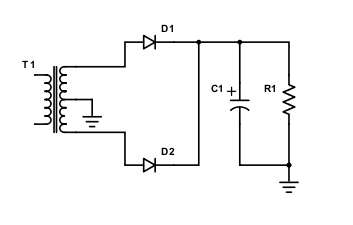
\includegraphics[height=3.5cm]{imgSource/circ1.png}
    \caption{Circuito retificador com capacitor associado à carga resistiva.}
    \label{fig:circ1}
\end{figure}

\begin{figure}[h!]
    \centering
    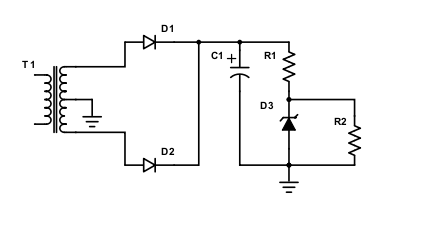
\includegraphics[height=3.5cm]{imgSource/circ2.png}
    \caption{Circuito retificador de onda completa regulado por diodo Zener.}
    \label{fig:circ2}
\end{figure}

\begin{figure}[h!]
    \centering
    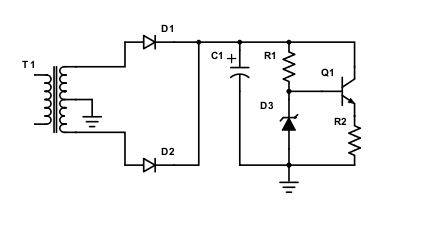
\includegraphics[height=3.5cm]{imgSource/circ3.png}
    \caption{Circuito retificador de onda completa regulado por diodo Zener e transistor.}
    \label{fig:circ3}
\end{figure}

\begin{figure}[h!]
    \centering
    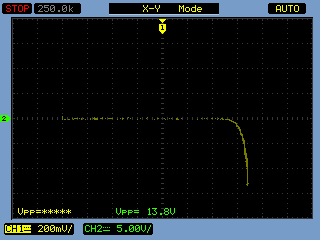
\includegraphics[height=5.5cm]{imgSource/tensaoDioxcorrRes.png}
    \caption{Gráfico de tensão no diodo por corrente no resistor.}
    \label{fig:tensaoxcorrente}
\end{figure}

\begin{figure}[h!]
    \centering
    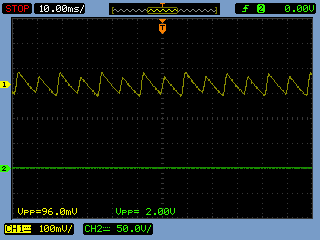
\includegraphics[height=5.5cm]{imgSource/rippleRet.png}
    \caption{Gráfico que mostra a tensão de ripple no circuito retificador.}
    \label{fig:rippleRet}
\end{figure}

\begin{figure}[h!]
    \centering
    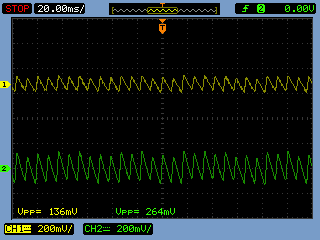
\includegraphics[height=5.5cm]{imgSource/rippleResMenor.png}
    \caption{Gráfico que mostra a tensão de ripple no circuito retificador com uma menor resistência de carga.}
    \label{fig:rippleResMenor}
\end{figure}

\begin{figure}[h!]
    \centering
    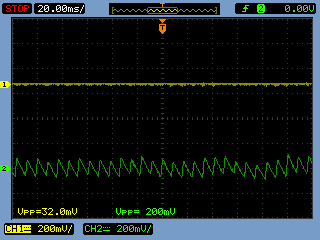
\includegraphics[height=5.5cm]{imgSource/zenerNoRipple.png}
    \caption{Gráfico que mostra a ausência de tensão de ripple no retificador feito com o diodo de zener.}
    \label{fig:zenerNoRipple}
\end{figure}

\begin{figure}[h!]
    \centering
    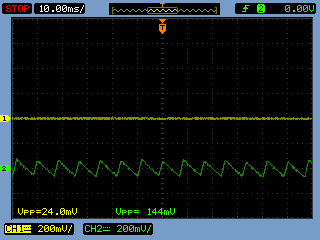
\includegraphics[height=5.5cm]{imgSource/zenerRipple.png}
    \caption{Gráfico que mostra a presença da tensão de ripple no retificador feito com o diodo de zener ao se alterar a resistência de carga.}
    \label{fig:zenerRipple}
\end{figure}

\begin{table}[h!]
    \label{tab: tensao-diodo}
    \begin{tabular}{|l|l|l|l|l|}
    V(V)   & $v_d$(V)   & $v_r$(V)   & i(mA)    & $r_d$($\Omega$)     \\
    9,3 & 0,67 & 8,59 & 6,61 & 101,39 \\
    6,2 & 0,6  & 5,45 & 4,19 & 143,12 \\
    3   & 0,6  & 2,4  & 1,85 & 325,67
    \end{tabular}
    \caption{Valores das tensões na fonte (V), no diodo comum ($v_d$), no resistor ($v_r$), corrente (i) e resistência do diodo ($r_d$) }
\end{table}

\begin{table}[h!]
    \label{tab: tensao-zener}
    \begin{tabular}{|l|l|l|l|l|}
    V(V)   & $v_d$(V)   & $v_r$(V)   & i(mA)    & $r_d$($\Omega$)     \\
    9,3 & 0,738 & 8,55  & 6,58 & 103,16 \\
    6,2 & 0,726 & 5,49  & 4,22 & 152,26 \\
    3,2 & 0,706 & 2,589 & 1,99 & 288,81
    \end{tabular}
    \caption{Valores das tensões na fonte (V), no diodo Zener ($v_d$), no resistor ($v_r$), corrente (i) e resistência do diodo ($r_d$) }
\end{table}

\end{document}
